% !TEX root = ../../main.tex
\chapter{Object Reconstruction and Identification}
\label{ch:objreco}

Combining measurements from various ATLAS subdetectors allows for the identification of physics objects like electrons, muons, photons, and hadrons. The trajectory of a particle can be reconstructed by matching position measurements in the calorimeters and MS with track hits in the ID. Converging tracks extrapolated towards the IP identify vertices, and the one with the largest $\sum \pT^2$ for all associated tracks is labeled the primary vertex (PV).  Reconstructed objects are associated to the same interaction when their tracks extrapolate to the PV. In this analysis, the reconstructed objects of interest are: electrons, muons and jets. Additionally, missing transverse energy, $\MET$, is used to identify neutrinos which do not interact with the detector. This chapter describes the selections and algorithms used to identify these physics objects.

%
\section{Electrons}
\label{ch:objreco:el}
Electron objects are reconstructed by matching clusters of EM calorimeter energy deposits to reconstructed tracks in the ID. To build the EM cluster, a sliding window algorithm is used~\cite{sliding_window}. The window is a fixed-size grid of cells, $N_{\eta}\times N_{\phi}$=3\times5, in the middle layer of the LAr calorimeter where approximately $80\,\%$\,of the energy in an EM shower is deposited (\Sect{\ref{ch:atlas:particle_showers}}). For each cell, the energy is summed across all the longitudinal layers, forming a tower. If the transverse energy of the towers in the window is above 2.5\,\GeV\,and is a local maximum, a seed cluster is formed. 

After loose shower shape requirements are applied to the seed clusters, a cone-shaped region of interest (ROI) of $\Delta R<0.3$ from the seed barycenter is defined~\cite{electron_efficiency, electron_efficiency_2016}.  Pattern recognition and track fitting algorithms are then used to match ID tracks to seed clusters. Track seeds from the ID with $\pT>1\,\GeV$\, are tested against pion and electron pattern recognition algorithms, and are required to reside in a cluster ROI. A track fit is performed twice to extrapolate the ID track to the calorimeter, using the track momentum or the cluster momentum, and is required to be near the cluster. If either succeeds, a final optimized track reconstruction is performed using a Gaussian Sum Fitter (GSF)~\cite{gsm_filter}. 
%A summary of the track reconstruction and cluster matching parameters is shown in~\Tab{\ref{tab:el_cl_tr}}.

An electron candidate is formed if there is at least one ID track matched to the seed cluster. The EM cluster is then rebuilt by summing energy in a grid of $3\times 7$ cells in each layer, starting in the middle layer. After calibrations and corrections are applied, the four-momentum of the electron candidate is calculated using the energy measurement of the EM cluster and the $\eta$ and $\phi$ measurements from the track.

%\begin{table}[tb]
%\begin{center}
%\begin{tabular}{l|c|c|c|c}
%\hline\hline
%\textbf{Reconstruction} & \multicolumn{2}{c|}{$\Delta\phi_{\textrm{EM cluster}}$} & \multicolumn{2}{c}{$\Delta\eta_{\textrm{EM cluster}}$}  \\\cline{2-5}
%\textbf{Method}& Curve toward & Curve away & non-TRT-only & TRT-only \\\hline
%Track Momentum & $<0.2$ & $<0.05$ & $<0.05$ & --- \\\cline{2-5}
%Cluster Momentum & $<0.1$ & $<0.05$ & $<0.05$ & --- \\\hline
%\multicolumn{1}{l}{\textbf{Final}} &\multicolumn{4}{c}{\,} \\\hline
%$\quad$ non-TRT-only (GSF) & \multicolumn{2}{c|}{$<0.1$} & \multicolumn{2}{c}{---} \\\cline{2-5}
%$\quad$ TRT-only & $<0.03$ & $<0.02$ & --- & $<0.35$\\\hline\hline
%\end{tabular}
%\caption[Calorimeter cluster track matching requirements]{Requirements on the proximity of the extrapolated tracks to the calorimeter cluster seeds are shown for several reconstruction methods. The $\Delta\phi$ requirements depend on if the reconstructed track curves toward or away from the seed cluster. If extrapolation with either the track momentum or cluster momentum succeeds, a final track reconstruction is performed. For non-TRT-only tracks, the final reconstruction uses an optimized Gaussian Sum Filter (GSF) algorithm~\cite{gsm_filter}. }
%\label{tab:el_cl_tr}
%\end{center}
%\end{table}



Background objects like hadronic jets, non-prompt electrons from photon conversions, and semi-leptonic decays of hadrons with heavy quarks can ``fake'' an electron signature and be reconstructed at this stage as an electron candidate~\cite{electron_efficiency}. A multivariate analysis (MVA) technique takes into account several cluster and track variables to create a likelihood (LH) identification for each candidate as either signal or background. Different working points balancing signal efficiency with background rejection are provided as shown in~\Fig{\ref{fig:el_id_eff}}; in this analysis, the ``LooseLH'' and ``TightLH'' are considered, where TightLH is a subset of LooseLH. The LooseLH working point has very high signal efficiency and mostly offers light flavor jet discrimination. The TightLH working point has a lower signal efficiency, but additionally rejects photon conversions and heavy flavor jets.

In addition to the discrimination due to the LH identification, further suppression of background electrons is provided with isolation criteria~\cite{electron_efficiency_2016}. A real electron from, for example, a $W$ boson decay, will be produced in relative isolation while jets, converted photons, and other fake electrons will be accompanied by nearby energy deposits. Isolation is calculated both from the calorimeter EM cluster, and from the ID track. Calorimeter isolation, $E_{\rm T}^{\textrm{cone} 0.2}$, calculates the sum of transverse energy ($E_{\rm T}$) in a cone of $\Delta R<0.2$ around the 
\begin{wrapfigure}{r}{.6\textwidth}
\begin{center}
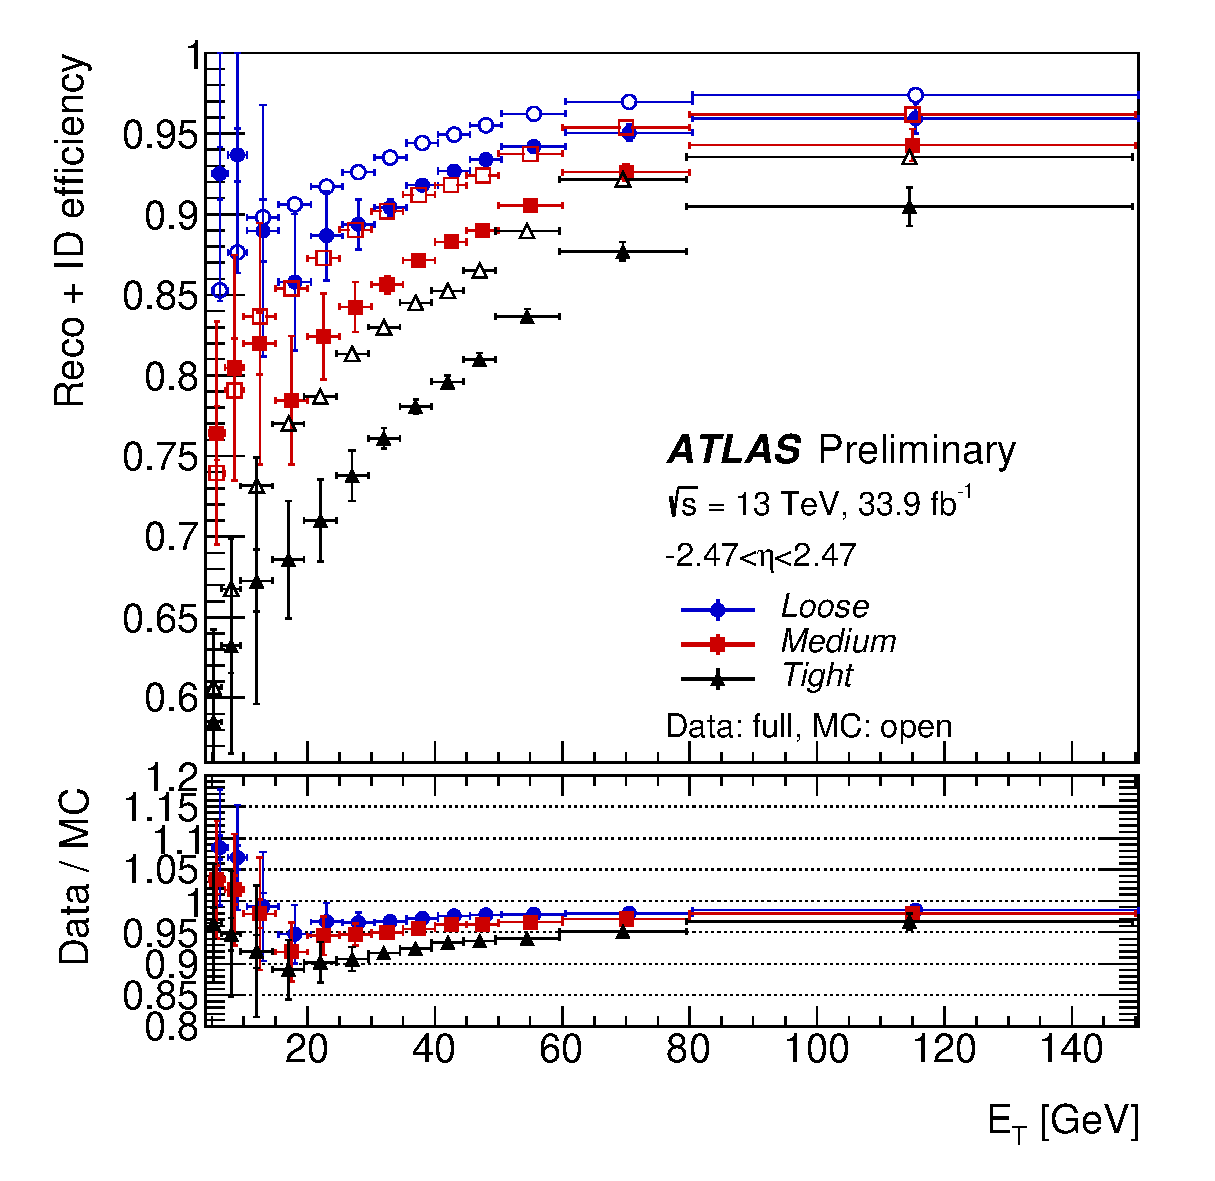
\includegraphics[width=.59\textwidth]{figures/ObjectReconstruction/el_id_eff}
\end{center}
\caption[Electron reconstruction and identification efficiencies]{The reconstruction and identification efficiencies for signal electrons is presented as a function of transverse energy for several working points~\cite{el_id_eff}.}
\label{fig:el_id_eff}
\end{wrapfigure}
electron center, and subtracts the $5\times7$ cell window contribution from the electron. Track isolation, $\pT^{\textrm{varcone} 0.2}$, calculates the sum of transverse momentum for quality tracks in a variable cone of size $\Delta R< \textrm{min}(0.2, 10\,\GeV/E_{\rm T})$ centered around and excluding the electron track. Working points using calorimeter and/or track based isolation are provided for either 1) a specific efficiency with variable cuts or 2) fixed cut values. The ``LooseTrackOnly'' and ``FixedCutTight'' isolation working points are used in this analysis. The LooseTrackOnly working point only uses the ID track based isolation for a constant $99\,\%$\, efficiency. The FixedCutTight working point cuts at $E_{\rm T}^{\textrm{cone} 0.2}/E_T < 0.06$ and $\pT^{\textrm{varcone} 0.2}/E_T < 0.06$.

The identification and isolation working points are optimized for electrons coming from the PV. This analysis additionally requires the recommended cuts on longitudinal ($z_0$) and transverse ($d_0$) impact parameters to verify the reconstructed electron is associated with the PV. Electrons are required to have $|\eta|<2.47$, excluding the calorimeter transition region between $1.37<|\eta|<1.52$, where the uncertainties can be large due to poor resolution. Finally, a minimum transverse momentum is required to avoid trigger turn-on curves, as discussed in~\Ch{\ref{ch:event_selection}}. This analysis uses two types of electrons, ``signal'' and ``veto'', which are defined and summarized in~\Tab{\ref{tab:lep_def}}. Veto electrons are used to avoid overlap with similar analyses with distinct final states. 

\begin{table}[htbp]
\begin{center}
\begin{tabular}{l|c|c|c|c}
\hline\hline
\multicolumn{1}{c|}{\textbf{Cut}} & \multicolumn{2}{c|}{\textbf{Electron Definition}} &  \multicolumn{2}{c}{\textbf{Muon Definition}} \\\cline{2-5}
& Veto & Signal & Veto & Signal \\\hline
\pt [\GeV] & $>7$ & $> 27$  & $>7$ & $> 27$ \\\hline
$|\eta|$ & \multicolumn{2}{c|}{$<2.47\notin[1.37, 1.52]$} & $<2.7$ & $<2.5$ \\\hline
Identification & LooseLH & TightLH & Loose & Medium  \\\hline
\vbox{\hbox{\strut Isolation}\hbox{\strut}} & \vbox{\hbox{\strut LooseTrack-}\hbox{\strut Only}} & \vbox{\hbox{\strut FixedCutTight}\hbox{\strut}} & \vbox{\hbox{\strut LooseTrack-}\hbox{\strut Only}} & \vbox{\hbox{\strut FixedCutTight-}\hbox{\strut TrackOnly}}\\\hline
$|d_0/\sigma(d_0)^{BL}|$ & \multicolumn{2}{c|}{$<5$} & \multicolumn{2}{c}{$<3$}\\\hline
$|z_0\sin\theta|$ [mm]& \multicolumn{4}{c}{$< 0.5$}  \\\hline\hline
\end{tabular}
\caption[Electron and muon object definitions]{The object definitions for electrons and muons used in this analysis are shown. Veto leptons are defined to reduce overlap with similar final state searches. }
\label{tab:lep_def}
\end{center}
\end{table}
%
\section{Muons}
Muon objects are reconstructed by matching track candidates independently created in the MS and ID~\cite{muon_eff}. In the MS, algorithms create segments by matching hits aligned in the bending plane between multiple layers. If multiple track segments match in different layers, a track candidate is formed. 

Using combinations of information from the ID, calorimeters, and MS, four types of muon candidates are defined. In decreasing priority, they are:
\begin{itemize}
	\item \underline{Combined (CB)}: The full muon track is reconstructed, starting in the MS and extrapolating towards the ID.
	\item \underline{Segment Tagged (ST)}: The ID track is extrapolated towards the MS, where it must match at least one MDT/CSC track segment (useful for low-\pT muons).
	\item \underline{Calo Tagged (CT)}: The ID track is extrapolated to the calorimeter, where it matches an energy deposit (useful in the region $|\eta|<0.1$ where the MS has no coverage).
	\item \underline{Stand Alone (SA)}: A MS track not matched to an ID track, but extrapolated close to the IP, is used to recover muons in the range $2.5<|\eta|<2.7$ that has poor ID coverage.
\end{itemize}

Background objects, such as decaying pions and kaons, can be reconstructed as a ``fake'' muon candidate. Using the four types of muon candidates, and additional cuts based on track and calorimeter based variables, working points for muon identification are created to balance signal efficiency with background rejection. In this analysis, the ``Medium'' and ``Loose'' identification working points are used, corresponding to approximate efficiencies of 96.1\,\% and 98.1\,\%, respectively. The Medium working point only uses CB and SA candidates, while the Loose working point considers all four types. 

Muon isolation is performed analogously to electron isolation: track-based and calorimeter-based isolation measurements are used to create working points with either 1) efficiency based variable cuts or 2) fixed cuts. The track-based muon isolation, $\pt^{\textrm{varcone} 0.3}$, uses a slightly larger cone, $\Delta R < 0.3$, with respect to the electron case.  In this analysis, ``LooseTrackOnly'' and ``FixedCutTightTrackOnly'' isolation working points are used. The LooseTrackOnly working point has a constant $99\,\%$\, efficiency. The FixedCutTightTrackOnly requires $\pt^{\textrm{varcone} 0.3}/\pT < 0.06$.

Finally, as with electrons, two types of muon objects are defined, ``signal'' and ``veto''. Recommended $\pT$, $\eta$, and PV association cuts are additionally placed on the muon objects, whose definitions are summarized in~\Tab{\ref{tab:lep_def}}. 

%
\section{Jets}
Hadronization of quarks from the initial hard scatter event, or subsequent hadronic decays of unstable particles ($W\ra q\overline{q}'$, $Z\ra q\overline{q}$), creates showers of lower energy particles, called jets, in the detector. Jets are formed by clustering nearby energy deposits in the calorimeter and matching the cluster with ID tracks. 

Topologically connected three dimensional cell clusters, or ``topo-clusters''~\cite{topo_cluster}, are used as constituents in the formation of a jet. Unlike the sliding-window calorimeter cluster seeds used for electrons, topo-clusters can have variable sizes. A topo-cluster is seeded if the energy of a cell is four standard deviations above the noise level ($E_{\textrm{cell}}>4 \sigma_{\textrm{cell}}^{\textrm{noise}}$), and connected cells are added to the cluster if $E_{\textrm{cell}}>2 \sigma_{\textrm{cell}}^{\textrm{noise}}$. 

The anti-$k_{\rm T}$ jet reconstruction algorithm~\cite{anti_kt_algo} is a sequential combination algorithm used in this analysis to combine topo-clusters into jet objects. A distance parameter is defined in~\Eqn{\ref{eq:anti_kt}}.
\begin{eqnarray}
\label{eq:anti_kt}
d_{ij} &=& \textrm{min}\left(\frac{1}{p_{\rm T,i}^2},\frac{1}{p_{\rm T,j}^2}\right)\frac{\Delta R_{ij}^2}{R^2}  \\
d_{iB} &=& \frac{1}{p_{\rm T,i}^2} 
\end{eqnarray}
The distance $d_{ij}$ measures the distance between two topo-clusters, while $d_{iB}$ measures the distance between a topo-cluster and the beam line. The distance parameter, $R$, roughly defines the size of the jet. The clustering procedure iteratively finds the smallest distance among all constituents. If the smallest distance is between two clusters, $d_{ij}$, the clusters are combined and the procedure continues. If it is between a cluster and the beam axis, $d_{iB}$, the cluster is defined as a jet and removed from the collection of remaining constituents. The distances are then recalculated and more jets are found until there are no remaining clusters. The anti-$k_{\rm T}$ algorithm tends to combine high-\pT constituents first and produces a roughly conical jet. ID tracks are matched with jets through a procedure known as ``ghost association''~\cite{ghost_assoc}. In effect, tracks are identified as particles with infinitesimal momentum and included in the clustering process. Their negligible momentum ensures the final jet clusters are not affected, but will include the tracks. In this analysis, ``small-R jets'' ($j$) and ``large-R jets'' ($J$), corresponding to $R=0.4$ and $R=1.0$, are used.

The energies of calorimeter jets are corrected for PU with a $\mu$-dependent subtraction. Additionally, a ``jet energy scale" (JES) response correction~\cite{jet_energy_measurement}  is applied to accurately calibrate both EM and hadronic showers. The JES aims to correct for the non-compensating nature of the calorimeters (hadrons have a lower detector response with respect to EM objects like electrons and photons), and energy loss in regions of the detector without measuring instruments. Small-R jets in this analysis use a simple JES scheme, called ``EM+JES'', in which the jets are measured at the EM scale\footnote{
	 The EM scale means the energy of an EM shower will be correctly measured.
} and a scale factor is applied based on the $\pT$ and $\eta$ measurements of the jet. For large-R jets, a local cluster weighting (LCW) procedure applies calibrations at a topo-cluster level, according to whether the cluster corresponds to a hadronic or EM energy deposit.  In this ``LCW+JES" scheme, jets are reconstructed from the locally calibrated clusters and a final JES scale factor is applied (smaller than in the EM+JES scheme). 
%
\subsection{Small-R Jets}
\label{ch:objectReconstruction:smallr}
Small-R jets ($R=0.4$) are used in this analysis to identify both VBF jets, and jets from $b$-quark decays. In VBF candidate events, the initial quarks, which radiate vector bosons, have a small deflection and hadronize into two jets with a large separation in $\eta$. Jets with $b$-hadrons, called $b$-jets, are useful for identifying candidate events from top quark pair decays ($t\bar{t}$). Candidate $b$-jets (VBF jets) must have $\pT>20\,\GeV$\, (30\,\GeV) and $|\eta| < 2.5$ (4.5).

Although a uniform PU subtraction is applied, local deviations may create PU jets. These jets can originate from both QCD effects (from a single PU vetex) and stochastic effects (contributions from multiple vertices). To reject both types of PU jets, a jet vertex tagger (JVT)~\cite{jvt} is used to assign jets to the PV. The JVT is a two-dimensional likelihood discriminant which factors in tracking and vertex information. For this analysis, the 92\,\% efficiency working point is used for jets with $\pT<60\,\GeV$\,and $|\eta|<2.4$. A residual 2\,\% of PU jets remain at this efficiency.

A multivariate $b$-tagging algorithm called MV2~\cite{b_jet} is used to tag small-R jets that contain $b$-hadrons. MV2 takes as input several $b$-tagging algorithms based on the impact parameter, secondary vertex reconstruction, and full decay chain reconstruction. The MV2 algorithm uses a boosted decision tree with background composition from $c$-jets (light-jets) of 7\,\% (93\,\%). Light-jets refer to jets from gluons or $u, d,$ or $s$ quarks. For this analysis, the 85\,\%\,efficiency $b$-tagging working point is used. The inverse of the corresponding mis-tag rate, called the rejection ratio, is 3.1 (33) for $c$-jets (light-jets)~\cite{b_jet_opt}. VBF candidate jets are required to fail $b$-tagging. A summary of the small-R jets definitions is shown in~\Tab{\ref{tab:small_j_def}}.

\begin{table}[htbp]
\begin{center}
\begin{tabular}{l|c|c}
\hline\hline
\multicolumn{1}{c|}{\textbf{Cut}} & \multicolumn{2}{c}{\textbf{Small-R Jet Definition}} \\\cline{2-3}
& $b$-jet Candidate & VBF jet Candidate  \\\hline
Algorithm & \multicolumn{2}{c}{Anti-$k_{\rm T}$ $R=0.4$}  \\\hline
Energy Calibration & \multicolumn{2}{c}{EM+JES} \\\hline
\pt [\GeV] &$>20$&$>30$\\\hline
$|\eta|$ &$<2.5$&$<4.5$\\\hline
\vbox{\hbox{\strut Pileup Removal}\hbox{\strut (JVT 92\,\% efficiency)}} & \multicolumn{2}{c}{\vbox{\hbox{\strut if\, $\pT<60\,\GeV$}\hbox{\strut \&\& $|\eta|<2.4$}}}  \\\hline
$b-$tag (MV2c10 85\,\% efficiency)& pass & fail \\\hline\hline
\end{tabular}
\caption[Small-R jet object definition]{The object definitions for small-R jets used in this analysis are shown.}
\label{tab:small_j_def}
\end{center}
\end{table}


%
\subsection{Large-R Jets}
\label{ch:objectReconstruction:larger}
Large-R jets ($R=1.0$) are used in this analysis to identify boosted hadronically decaying vector bosons.  Jets from the two-body decays of boosted vector bosons have a substructure typically absent from decays of gluons and light quarks~\cite{boost_trim}. To elucidate the substructure differences, grooming techniques remove soft contributions to the jet. In particular, this analysis uses a grooming technique called trimming, depicted in~\Fig{\ref{fig:jet_trim}}. Jet trimming further aims to improve the jet mass resolution by removing contamination from initial state radiation (radiation from the incoming hadrons), multiple parton interactions (further interactions among the partons after the hadron collision), and PU interactions. 
The trimming procedure in this analysis involves the following steps:
\begin{itemize}
	\item Re-cluster the large-R jet ($J$) constituents into ``sub-jets'' with the anti-$k_{\rm T}$ algorithm with distance parameter $R=0.2$.
	\item Remove sub-jets if $p_{\rm T}^{\textrm{sub-jet}}< 0.05\times p_{\rm T}^{J}$.
	\item Recombine the surviving sub-jets into a final trimmed jet.
\end{itemize}
\begin{figure}[tbp]
\begin{center}
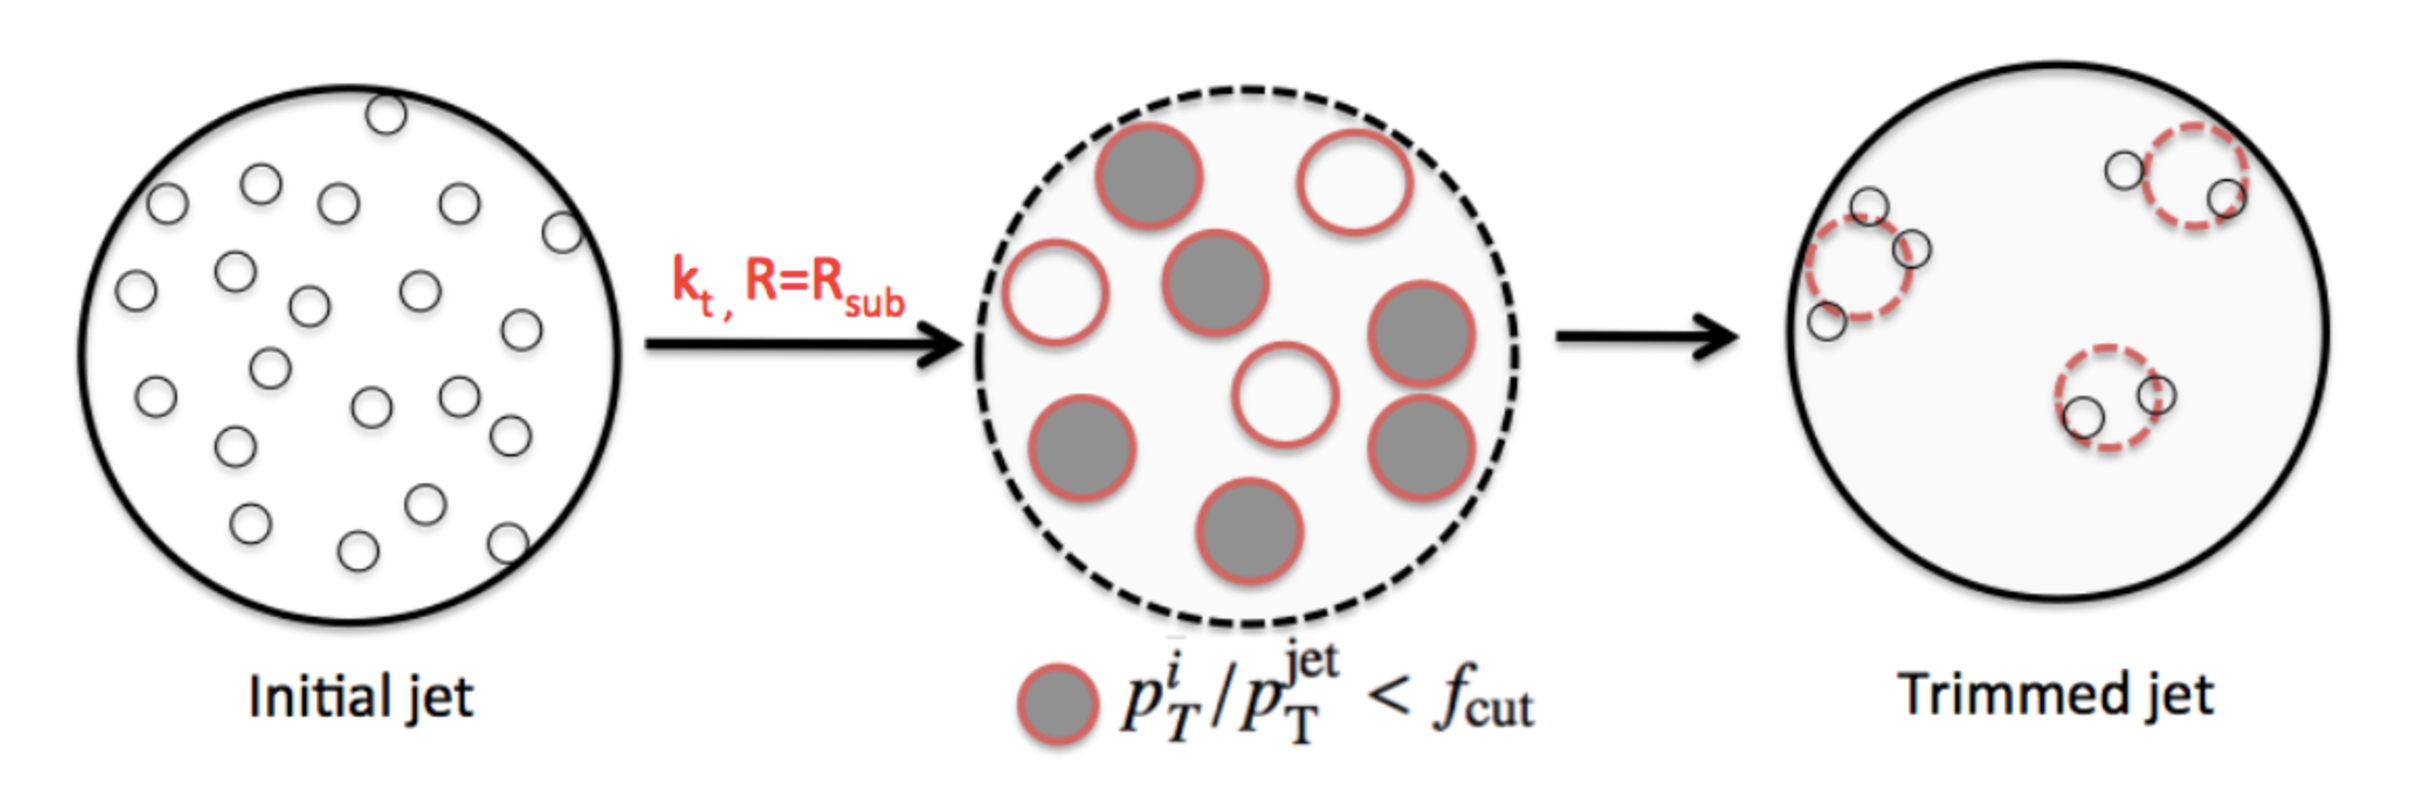
\includegraphics[width=.8\textwidth]{figures/ObjectReconstruction/jet_trim}
\caption[Jet trimming illustration]{The jet trimming procedure is illustrated. In this analysis, sub-jets are created with the anti-$k_{\rm T}$ algorithm with distance parameter $R_{\textrm{sub}}=0.2$, and the fractional \pT threshold is set at $f_{\textrm{cut}}=0.05$~\cite{boost_trim}.}
\label{fig:jet_trim}
\end{center}
\end{figure}

Even with trimming, jet mass resolution can suffer in the high-\pT regime from a loss of angular information when multiple highly boosted decay products are reconstructed as a single topo-cluster. A track mass, $m_{\textrm{track}}$, based on ID charged particle tracks can be used to improve the mass resolution~\cite{jet_track_mass}. The track mass is calculated by ghost associating ID tracks with $\pT>0.4\,\GeV$ to the large-R jet, and then summing the masses associated with all matched tracks. To correct for the missing neutral particle contribution to $m_{\textrm{track}}$, a ratio of the calorimeter-based to track-based transverse momentum is applied to the track mass. The resulting quantity, called the track-assisted mass, is shown in~\Eqn{\ref{eq:m_ta}}.
\begin{equation}
m_{\textrm{TA}} \equiv m_{\textrm{track}}\times\frac{p_{\rm T}^{\textrm{calo}}}{p_{\rm T}^{\textrm{track}}}
\label{eq:m_ta}
\end{equation}

To take advantage of both the calorimeter and track-assisted mass, a weighted sum, minimizing the jet mass resolution and called the combined mass, is defined in~\Eqn{\ref{eq:m_comb}}~\cite{jet_comb_mass}.
\begin{equation}
m_{\textrm{comb}} \equiv w_{\textrm{calo}}\times m_{\textrm{calo}} + w_{\textrm{track}}\times m_{\textrm{TA}}
\label{eq:m_comb}
\end{equation}
In this analysis, $m_{\textrm{calo}}$ and $m_{\textrm{TA}}$ are taken to be uncorrelated (reflecting an approximate 10\,\%\,correlation for $\pT > 1\,\TeV$). The weights in~\Eqn{\ref{eq:m_comb}} can thus be expressed in terms of the estimated jet mass resolution, $\sigma_{\textrm{calo}}$ ($\sigma_{\textrm{TA}}$) for $m_{\textrm{calo}}$ ($m_{\textrm{TA}}$), as shown in~\Eqn{\ref{eq:m_comb_uncorr}}.
\begin{equation}
m_{\textrm{comb}} = \frac{\sigma_{\textrm{calo}}^{-2}m_{\textrm{calo}} +  \sigma_{\textrm{TA}}^{-2}m_{\textrm{TA}}}{\sigma_{\textrm{calo}}^{-2}+\sigma_{\textrm{TA}}^{-2}}
\label{eq:m_comb_uncorr}
\end{equation}
The estimated jet mass resolutions are calculated as a function of \pT and $\eta$. The improvement in jet mass resolution of the combined mass is shown in~\Fig{\ref{fig:m_comb_res}}. The jet transverse momentum is also re-scaled to be compatible with the combined mass, as shown in~\Eqn{\ref{eq:jet_pt_comb}}.
\begin{equation}
p_{\rm T}^{\textrm{comb}} \equiv p_{\rm T}^{\textrm{calo}}\times\frac{m_{\textrm{comb}}}{m_{\textrm{calo}}}
\label{eq:jet_pt_comb}
\end{equation}
In the rest of this thesis, the combined mass and combined transverse momentum of the large-R jet will be referred to as $m(J)$ and $\pT(J)$ respectively. To ensure a complementary overlap between calorimeter and tracking information, large-R jets are required to have $|\eta|<2.0$. This search focuses on boosted $W$ or $Z$ bosons; thus, the large-R jet is required to have $\pT(J)>200\,\GeV$ and $m(J)>50\GeV$.
\begin{figure}[tbp]
\begin{center}
\subfloat[]{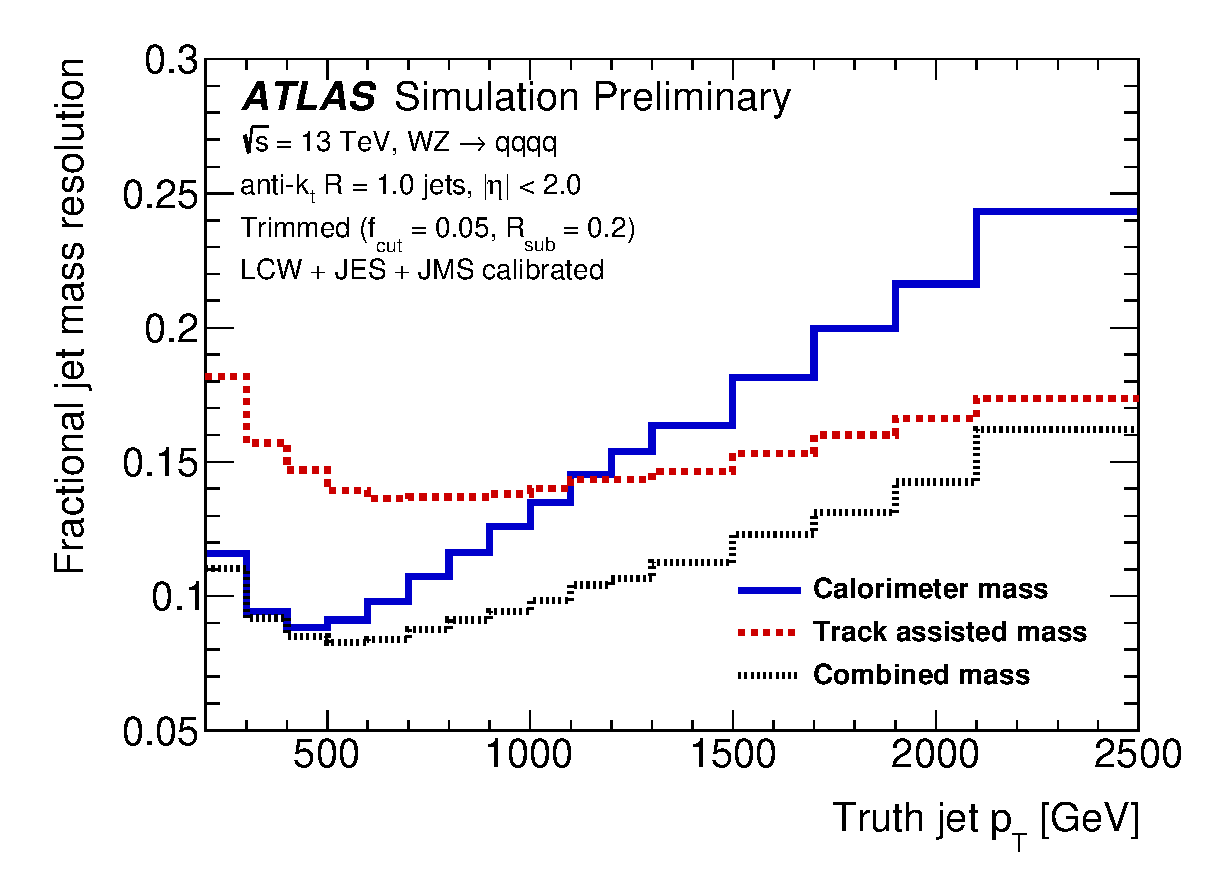
\includegraphics[width=.49\textwidth]{figures/ObjectReconstruction/m_comb_res}\label{fig:m_comb_res:a}}
\subfloat[]{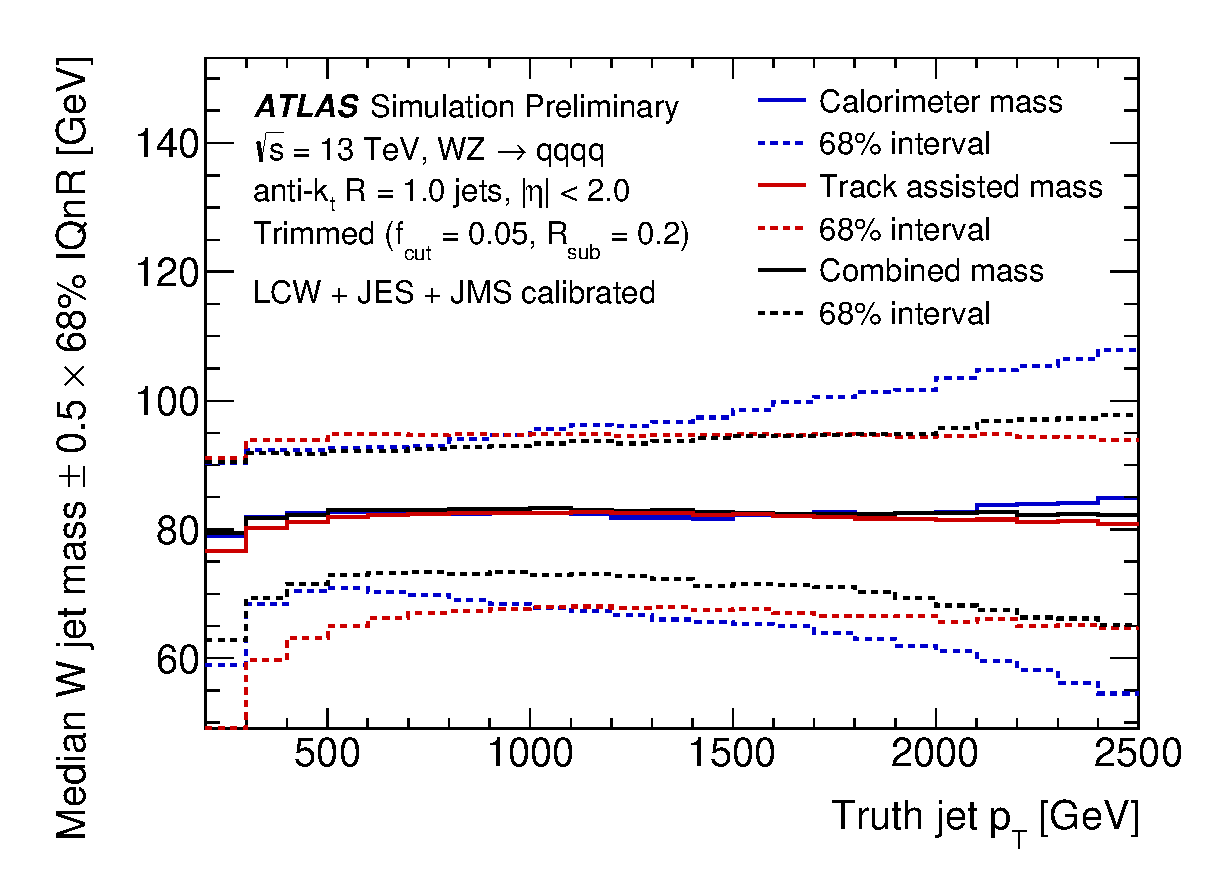
\includegraphics[width=.49\textwidth]{figures/ObjectReconstruction/med_reconst_w_mass}\label{fig:m_comb_res:b}}
\end{center}
\caption[Performance of combined mass for large-R jets]{Three jet mass definitions are used to compare \protect\subref{fig:m_comb_res:a} the fractional jet mass resolution and \protect\subref{fig:m_comb_res:b} the median reconstructed jet mass, for simulated boosted $W$ or $Z$ bosons, as a function of truth \pT. The combined mass improves jet mass resolution for $250\,\GeV<\pT<2.5\,\TeV$ and $|\eta|<2.0$~\cite{jet_track_mass}.}
\label{fig:m_comb_res}
\end{figure}


To further differentiate jets due to a two-body decay of boosted $W$ or $Z$ bosons from QCD jets due to single partons, a substructure variable ($D_2^{\beta=1}$), based on the ratio of generalized two and three point energy correlation functions, is introduced~\cite{d2_one, d2_two}, as shown in~\Eqnrange{\ref{eq:en_corr_func}}{\ref{eq:d2_def}}. 
\begin{eqnarray}
e_2^{\beta} & = & \frac{1}{\pT^2(J)}\sum_{1\leq i<j\leq n_j}\pT^i\pT^j\Delta R_{ij}^{\beta}  \label{eq:en_corr_func} \\
e_3^{\beta} & = & \frac{1}{\pT^2(J)}\sum_{1\leq i<j<k\leq n_j}\pT^i\pT^j\pT^k\Delta R_{ij}^{\beta}\Delta R_{ik}^{\beta}\Delta R_{jk}^{\beta} \\
D_{2}^{\beta=1} & = & \frac{e_3^{\beta=1}}{\left(e_2^{\beta=1}\right)^3} \label{eq:d2_def}
\end{eqnarray}
For $n_j$ constituents in the jet, $\pT^i$ is the transverse momentum of the i$^{\textrm{th}}$ constituent, and $\Delta R_{ij}$ is the previously defined angular separation between the i$^{\textrm{th}}$ and j$^{\textrm{th}}$ constituents.

A boson tagging algorithm, called SmoothedWZTagger~\cite{smoothed_wz_tagger}, identifies large-R jets as either a $W$ or $Z$ boson decay, based on the large-R jet combined mass and $D_2^{\beta=1}$ substructure variable, at fixed signal efficiency working points of $50\,\%$\, and $80\,\%$. The selections are optimized in \pT bins and a smoothing function is fit to the resulting mass-window and $D_2^{\beta=1}$ threshold cuts, as depicted in~\Fig{\ref{fig:smooth_cuts}}. A summary of the large-R jet definition is presented in~\Tab{\ref{tab:large_jet_def}}.
\begin{figure}[htbp]
\begin{center}
\subfloat[]{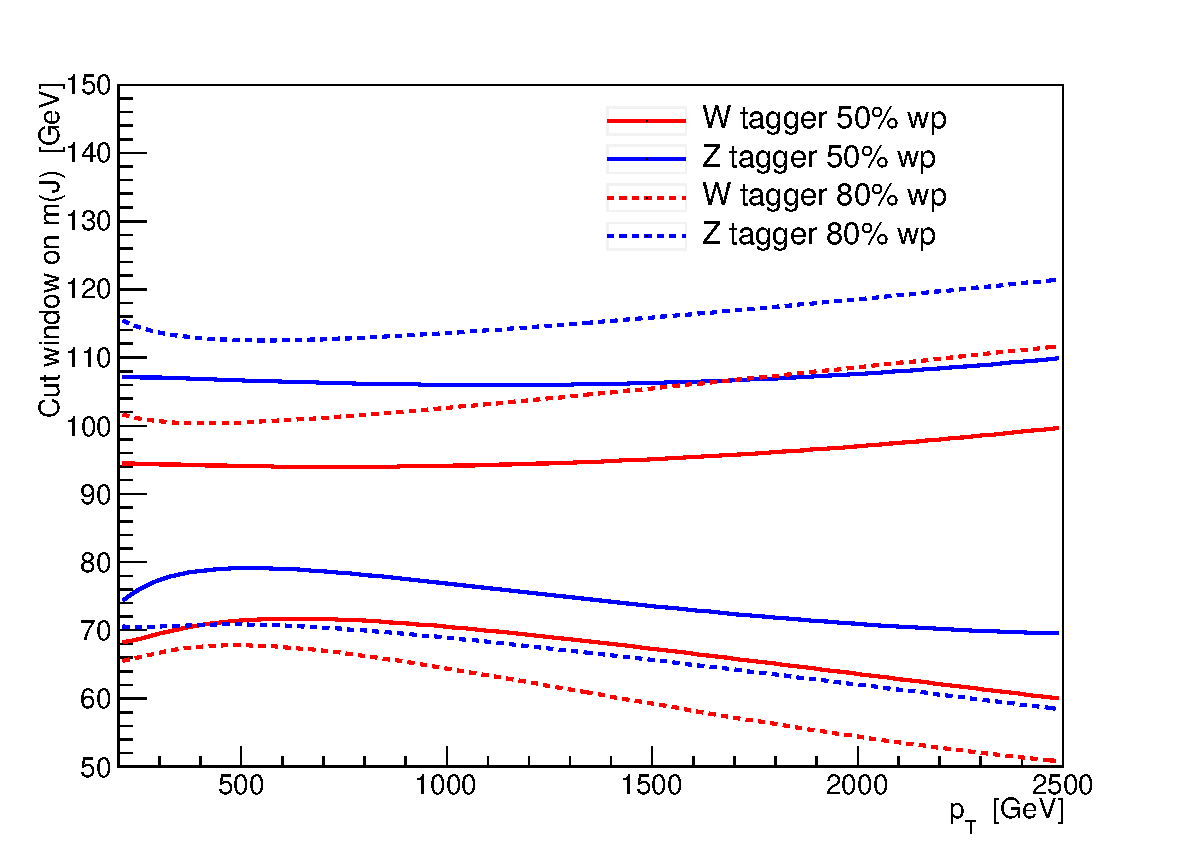
\includegraphics[width=.5\textwidth]{figures/ObjectReconstruction/MassWindow_newWZTagger}\label{fig:smooth_cuts:a}}
\subfloat[]{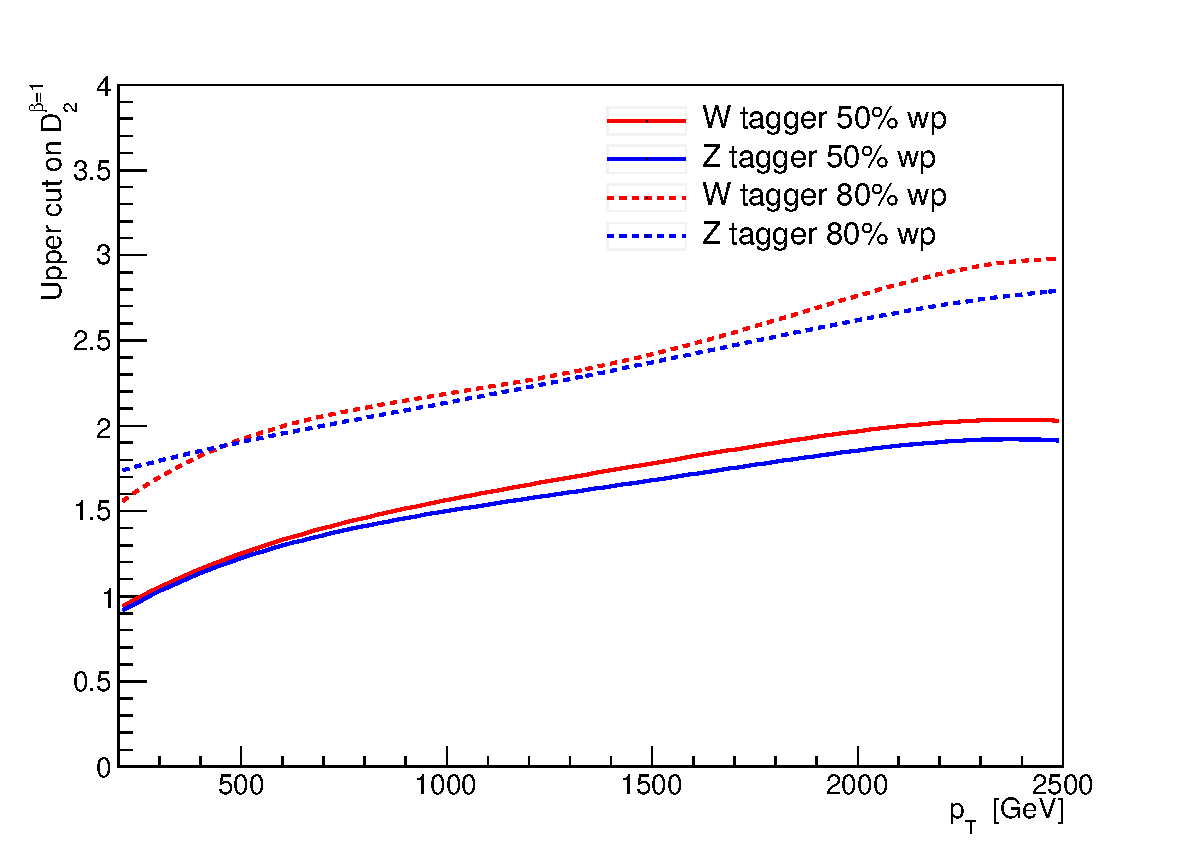
\includegraphics[width=.5\textwidth]{figures/ObjectReconstruction/D2UpperCut_newWZTagger}\label{fig:smooth_cuts:b}}
\caption[Boson tagger mass and substructure cuts]{The SmoothedWZTagger selections cuts for \protect\subref{fig:smooth_cuts:a} the combined mass window and \protect\subref{fig:smooth_cuts:b} the upper-cut on $D_2^{\beta=1}$, are shown as a function of \pT for both the $50\,\%$\,and $80\,\%$ efficiency working points. The $50\,\%$\,($80\,\%$) efficiency working point corresponds to a background rejection factor of 45-75 (11-13) and 50-70 (9-13) for $W$ and $Z$ bosons respectively.}
\label{fig:smooth_cuts}
\end{center}
\end{figure}
\begin{table}[htbp]
\begin{center}
\begin{tabular}{l|c}
\hline\hline
\textbf{Cut} &\textbf{Large-R Jet Definition} \\\hline
Algorithm & Anti-$k_{\rm T}$ $R=1.0$  \\\hline
Grooming & Trimming with $R_{\textrm{sub-jet}}=0.2$, $f_{\textrm{cut}}=0.05$ \\\hline
Energy Calibration & LCW+JES \\\hline
\pt [\GeV] &$>200$\\\hline
$|\eta|$ &$<2.0$\\\hline
Mass [\GeV] & $>50$ \\\hline
Boson Tagging & SmoothedWZTagger \\\hline\hline
\end{tabular}
\caption[Large-R jet definition]{The object definition for large-R jets used in this analysis.}
\label{tab:large_jet_def}
\end{center}
\end{table}


%
\section{Missing Transverse Energy}

Neutrinos produced in collisions pass through ATLAS without leaving energy deposits in the calorimeters, or tracks in the ID and MS. Since the colliding protons have no initial momentum transverse to the beam line, momentum conservation implies that the vector sum of the transverse momentum of all the final state particles should also be zero. Deviations from zero can indicate the presence of a non-interacting particle, like a neutrino, in the final state.  In \Eqn{\ref{eq:met_eq}}, the calculation of \MET is summarized as the negative vector sum of all reconstructed objects, and additional ``soft terms'' corresponding to tracks from the PV that are not matched to reconstructed objects.
\begin{eqnarray}
E^{\textrm{miss}}_{x(y)} &=& - \sum\limits_{e\in\{\textrm{electrons}\}} p_{x(y)}^{e}  - \sum\limits_{\mu\in\{\textrm{muons}\}} p_{x(y)}^{\mu}  - \sum\limits_{j\in\{\textrm{jets}\}} p_{x(y)}^{j}   - \sum\limits_{s\in\{\textrm{soft terms}\}} p_{x(y)}^{s} \nonumber \\
\MET & = & \sqrt{\left(E_x^{\textrm{miss}}\right)^2+ \left(E_y^{\textrm{miss}}\right)^2}
\label{eq:met_eq}
\end{eqnarray}
The use of soft terms that have ID tracks consistent with the PV ignores possible contributions from neutral particles. A calorimeter-based soft term, using topologically connected clusters unassociated with reconstructed particles, can be used to measure these contributions. However, the track-based soft terms offer better \MET resolution and are less pile-up dependent~\cite{met_perf}. As a result, the track-based soft terms are used in this analysis to reconstruct \MET. Photons and hadronically decaying taus are not used in this analysis, and are reconstructed as jets in the \MET calculation. 

In this analysis, the \MET is identified as the transverse momentum of the neutrino, $\pT^{\nu}$. To determine the $z$ component of the neutrino momentum, the $W$ boson from the $W\ra\ell\nu$ decay is constrained to be exactly on-shell with $m(W\ra\ell\nu)=80.4\,\GeV$. Using this constraint, a quadratic equation for the neutrino $p_z$ can be solved. If a solution is complex, the real part is taken, and if two unique solutions exist, the smallest in absolute value is taken. A more detailed discussion is presented in~\App{\ref{ch:neutrinopz}}.

%
\section{Overlap Removal}
As electrons, muons, and jets use a combination of tracking and calorimeter measurements, a single collection of energy deposits and tracks may be reconstructed independently as several physics objects. To remove any ambiguity, a procedure is defined to prioritize which reconstructed objects are kept and which are discarded.

\begin{itemize}
\item If there is a shared ID track between an electron candidate and a muon candidate, the electron is removed. In this case, the MS track from the muon candidate cannot be due to an electron. 
\item Next, if there is a small-R jet and electron candidate with $\Delta R(j,e)<0.2$, the small-R jet is removed since the reconstructed jet does not differentiate between hadronic and EM showers. However, the electron is removed if $0.2<\Delta R(j,e)<\textrm{min}(0.4,0.04+10\,\GeV/\pT(e))$. Electrons reconstructed near the edge of a jet are most likely from non-prompt decays of jet constituents. The sliding cone, with maximum size $R=0.4$ at low $\pT(e)$, recovers boosted prompt electrons that are close to the edge of jets. 
\item If there is a large-R jet and electron with $\Delta R(J,e)<1.0$, the large-R jet is removed. 
\item If a muon and small-R jet satisfy $\Delta R(j,\mu)<0.2$, and either 1) the jet has fewer than two tracks or 2) $\pT(\mu)/\pT(j)>0.5$ and $\pT(\mu)/\sum\pT(\textrm{tracks})>0.7$, the jet is discarded. This indicates the jet is most likely from the calorimeter energy loss of a muon. If the jet is not removed, a sliding cone is used to remove the muon if $\Delta R(j,\mu)<\textrm{min}(0.4,0.04+10\,\GeV/\pT(\mu))$. Similar to the electron case, boosted muons sufficiently far from the jet center are kept, while lower \pT muons likely from non-prompt decays near the jet edge are removed. 
\item There is no overlap removal between muons and large-R jets, as muons are unlikely to deposit enough calorimeter energy to be reconstructed as a jet with $\pT>200\,\GeV$.
\end{itemize}

